% ------------------------------------------------------------------------------
% 8.1. IMPLEMENTACIÓN DE LA ARQUITECTURA DEL SISTEMA
% ------------------------------------------------------------------------------
\wfa{\wn{8}.1. Implementación de la Arquitectura del Sistema}\label{sec:cap8_arquitectura_sistema}

Este capítulo describe cómo quedó construido el sistema ComedorUAGRM a partir del código desarrollado. La arquitectura diseñada en el capítulo 7 se conserva: clientes web y móvil, una API REST en Spring Boot organizada en seis paquetes funcionales, un módulo de preselección en Python y una base de datos PostgreSQL. Los diagramas de componentes del capítulo se elaboraron en Sparx Enterprise Architect y reflejan las clases reales del código.

El sistema se implementó como una aplicación cliente-servidor en capas, desplegada con Docker Compose. Los clientes son el panel web (React y TypeScript), la aplicación móvil (Flutter) y la landing institucional de Nexware (Astro). El tráfico HTTP del navegador pasa por un proxy inverso nginx que sirve el panel en la raíz, la landing en \texttt{/landing-page} y la API en \texttt{/api/}. El software central es la API REST \texttt{comedor-uagrm-core} (Java 21 y Spring Boot 4.1), organizada en los seis subsistemas definidos en el análisis. Esta API consume el módulo de IA \texttt{comedor-uagrm-ia} (Python y FastAPI), accesible solo desde ella por la red interna, y los servicios externos de correo (SMTP) y Firebase Cloud Messaging.

Los datos residen en PostgreSQL 18, con una base transaccional (OLTP) de 31 tablas gestionada con migraciones Flyway. El tablero de indicadores BI no usa un almacén OLAP ni cubos: se alimenta de cinco vistas materializadas de la misma base (\texttt{mv\_indicadores\_convocatoria}, \texttt{mv\_bi\_convocatoria}, \texttt{mv\_bi\_asistencia\_dia}, \texttt{mv\_bi\_carrera\_convocatoria} y \texttt{mv\_bi\_puntaje\_convocatoria}), que se refrescan periódicamente. Los archivos (documentos adjuntos, actas y planillas en PDF) se almacenan en MinIO, compatible con S3. Redis se emplea como caché únicamente en el caso de uso CU12 (dashboard de indicadores BI).

La Figura~\ref{fig:impl_sistema} presenta el diagrama de componentes del sistema completo: los seis paquetes de subsistemas con los casos de uso que los conforman, el software central, la base de datos transaccional (OLTP), las vistas de indicadores BI, el módulo de IA, MinIO y Redis. Los paquetes se relacionan según el flujo del proceso: becados y asistencia utiliza auditoría y adjudicación, esta utiliza convocatoria y postulación, y esta última utiliza preselección con IA. La Tabla~\ref{tab:impl_subsistemas} resume los casos de uso de cada subsistema.

\begin{table}[H]
\caption{Subsistemas y casos de uso que los conforman}
\label{tab:impl_subsistemas}
\centering
\footnotesize\linespread{1}\selectfont
\renewcommand{\arraystretch}{1.3}
\begin{tabular}{>{\raggedright\arraybackslash}p{5.5cm}>{\raggedright\arraybackslash}p{9.5cm}}
\toprule
\textbf{Subsistema} & \textbf{Casos de uso} \\
\midrule
Cuentas y Acceso & CU01, CU14, CU15 \\
Convocatoria y Postulación & CU13, CU02, CU16, CU17, CU18, CU04 \\
Preselección con IA & CU03, CU26 \\
Auditoría y Adjudicación & CU05, CU06, CU07, CU08, CU19, CU20, CU21, CU22 y el servicio de notificaciones (CU-EXTRA-01) \\
Becados y Asistencia & CU23, CU09, CU10, CU11, CU24 \\
Reportes y Trazabilidad & CU12, CU25 \\
\bottomrule
\end{tabular}

\smallskip
\noindent\raggedright\textit{Nota.} Elaboración propia.
\end{table}

\begin{landscape}
\begin{figure}[p]
\caption{Diagrama de Componentes de la Implementación de la Arquitectura del Sistema}
\label{fig:impl_sistema}
\centering
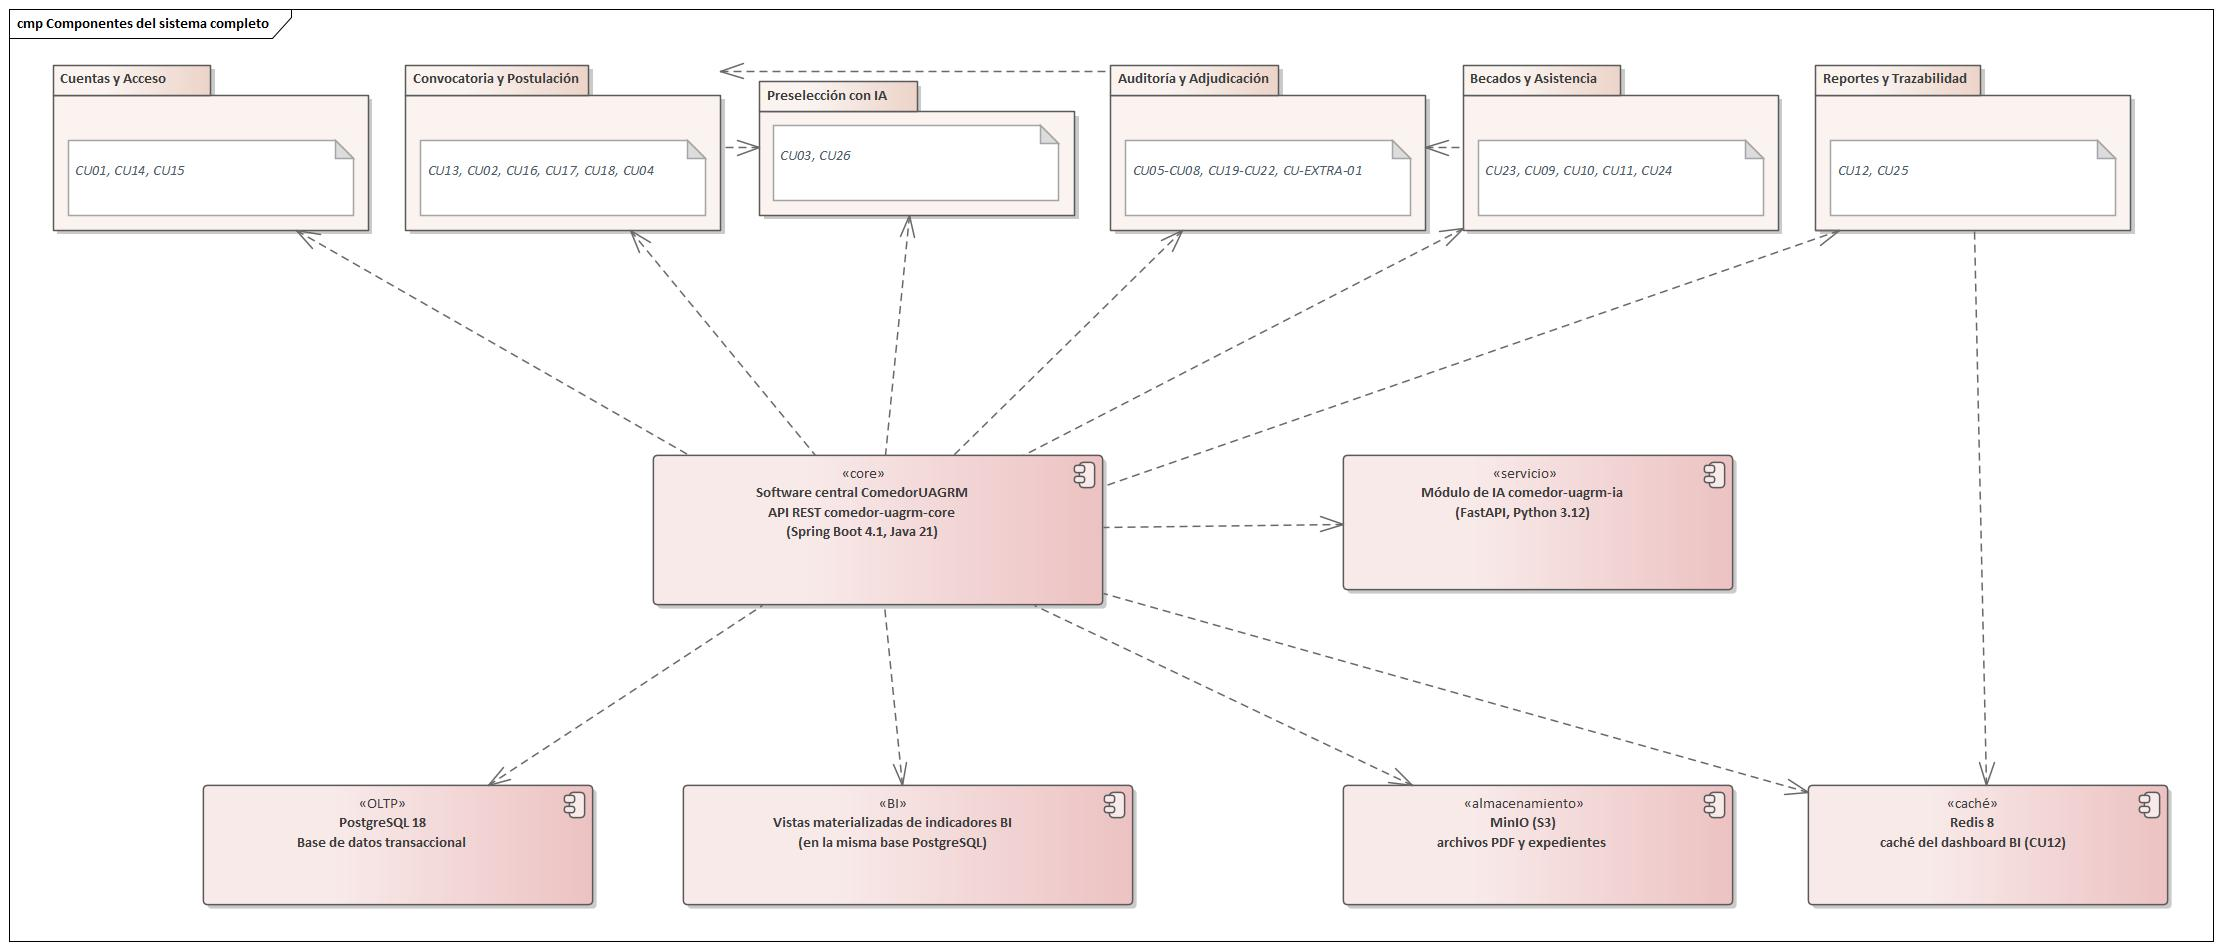
\includegraphics[width=\linewidth,height=0.8\textheight,keepaspectratio]{images/147_Componentes_Sistema_Completo.jpg}

\smallskip
\noindent\raggedright\textit{Nota.} Elaboración propia.
\end{figure}
\end{landscape}

